\documentclass[10pt]{beamer}

\usepackage{cmap}
\usepackage[T2A]{fontenc}
\usepackage[utf8]{inputenc}
\usepackage{amsfonts}
\usepackage{amsthm}
\usepackage{mathtools}
\usepackage{color}
\usepackage{hyperref}
\usepackage{graphicx}
\usepackage{pdfpages}
\usepackage{forest}
\usepackage{adjustbox}
\usepackage{times}
\usepackage{tikz}
\usetikzlibrary{decorations.pathreplacing}  % Подключение библиотеки для декораций
\usetikzlibrary{snakes,decorations.pathmorphing}


\mode<presentation>{
    \usetheme{Marburg}
    \usecolortheme{sidebartab}
}

% \newtheorem{theorem}{Theorem}[section]
% \newtheorem{lemma}{Lemma}[section]
% \newtheorem{proposition}{Proposition}[section]
% \newtheorem{corollary}{Corollary}[section]
% \newtheorem{definition}{Definition}[section]
% \newtheorem{remark}{Remark}[section]
% \newtheorem{example}{Example}[section]

\newcommand{\E}{\ensuremath{\mathbb{E}}}
\newcommand{\D}{\ensuremath{\mathbb{D}}}
\newcommand{\C}{\ensuremath{\mathbb{C}}}
\newcommand{\R}{\ensuremath{\mathbb{R}}}
\newcommand{\Q}{\ensuremath{\mathbb{Q}}}

\newcommand{\red}[1]{\textcolor{red}{#1}}
\newcommand{\blue}[1]{\textcolor{blue}{#1}}
\newcommand{\green}[1]{\textcolor{green}{#1}}
\newcommand{\orange}[1]{\textcolor{orange}{#1}}
\newcommand{\teal}[1]{\textcolor{teal}{#1}}
\newcommand{\purple}[1]{\textcolor{purple}{#1}}

\renewcommand{\phi}{\varphi}
\renewcommand{\epsilon}{\varepsilon}
\renewcommand{\le}{\leqslant}
\renewcommand{\ge}{\geqslant}

\begin{document}
    \title[NN-based pricing]{Прайсинг деривативов с помощью ML}
    \author{УРМ}
    \date{\today}
    \institute{Sber}

    \begin{frame}
        \titlepage
    \end{frame}

    \section{Что такое дериватив?}
    \begin{frame}{Что такое дериватив?}
        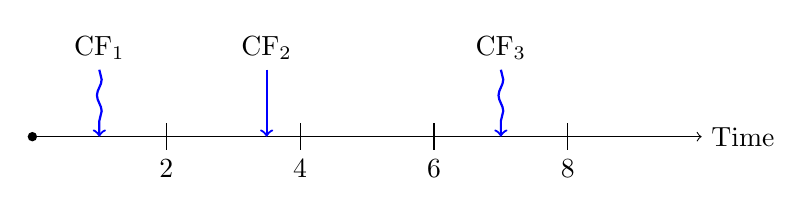
\begin{tikzpicture}[scale=0.85]  % Масштабирование всей картинки
            decoration={snake, amplitude=6mm, segment length=4mm}
            % Ось времени
            \fill[black] (0,0) circle (2pt); % Жирная точка в нуле
        \draw[->] (0,0) -- (10,0) node[right] {Time}; % Линия оси времени
    
            % Отметки на оси времени
            \foreach \x in {2, 4, 6, 8} {
                \draw (\x,0.2) -- (\x,-0.2) node[below] {\x};
            }
            
            % Волнистые стрелки
            \draw[decorate,decoration={snake, amplitude=0.3mm, segment length=4mm, post length=0.5mm},->,thick,blue] (1,1) -- (1,0);
            \draw[decorate,decoration={snake, amplitude=0mm, segment length=4mm, post length=0.5mm},->,thick,blue] (3.5,1) -- (3.5,0);
            \draw[decorate,decoration={snake, amplitude=0.3mm, segment length=4mm, post length=0.5mm},->,thick,blue] (7,1) -- (7,0);
            
            % Подписи для cashflow
            \node[above] at (1,1) {CF$_1$};
            \node[above] at (3.5,1) {CF$_2$};
            \node[above] at (7,1) {CF$_3$};
        \end{tikzpicture}
    \end{frame}

\end{document}